Grebogi y colaboradores \cite{Grebogi1988} han estudiado cómo el período $T$ se relaciona con la precisión.
Allí vieron que el período $T$ escala con el redondeo $\epsilon$ como $T \sim \epsilon^{-d/2}$ donde $d$ es la dimensión de correlación del atractor caótico.

Nagaraj \textit{et al.} \cite{Nagaraj2008} estudió el caso de la conmutación entre dos mapas.
Vieron que el período $T$ del mapa compuesto obtenido al conmutar entre dos mapas caóticos es más alto que el período de cada mapa y encontraron que una conmutación aleatoria mejora los resultados.
Aquí hemos considerado el solo la conmutación secuencial para evitar el uso de otra variable aleatoria, ya que esta puede introducir sus propias propiedades estadísticas en la serie temporal.

La Fig. \ref{fig:period} muestra $T$ vs. $B$ en escala semi logarítmica para el mapa logístico.
Los puntos promediados experimentales se pueden ajustar por una línea recta expresada como $\log_2 T = mB + b$ donde $m$ es la pendiente y $b$ es la ordenada al orígen.
Los resultados para todos los mapas considerados se resumen en la tabla \ref{tabla:periodos}.
%
\begin{figure}[htpb]
\centering	
	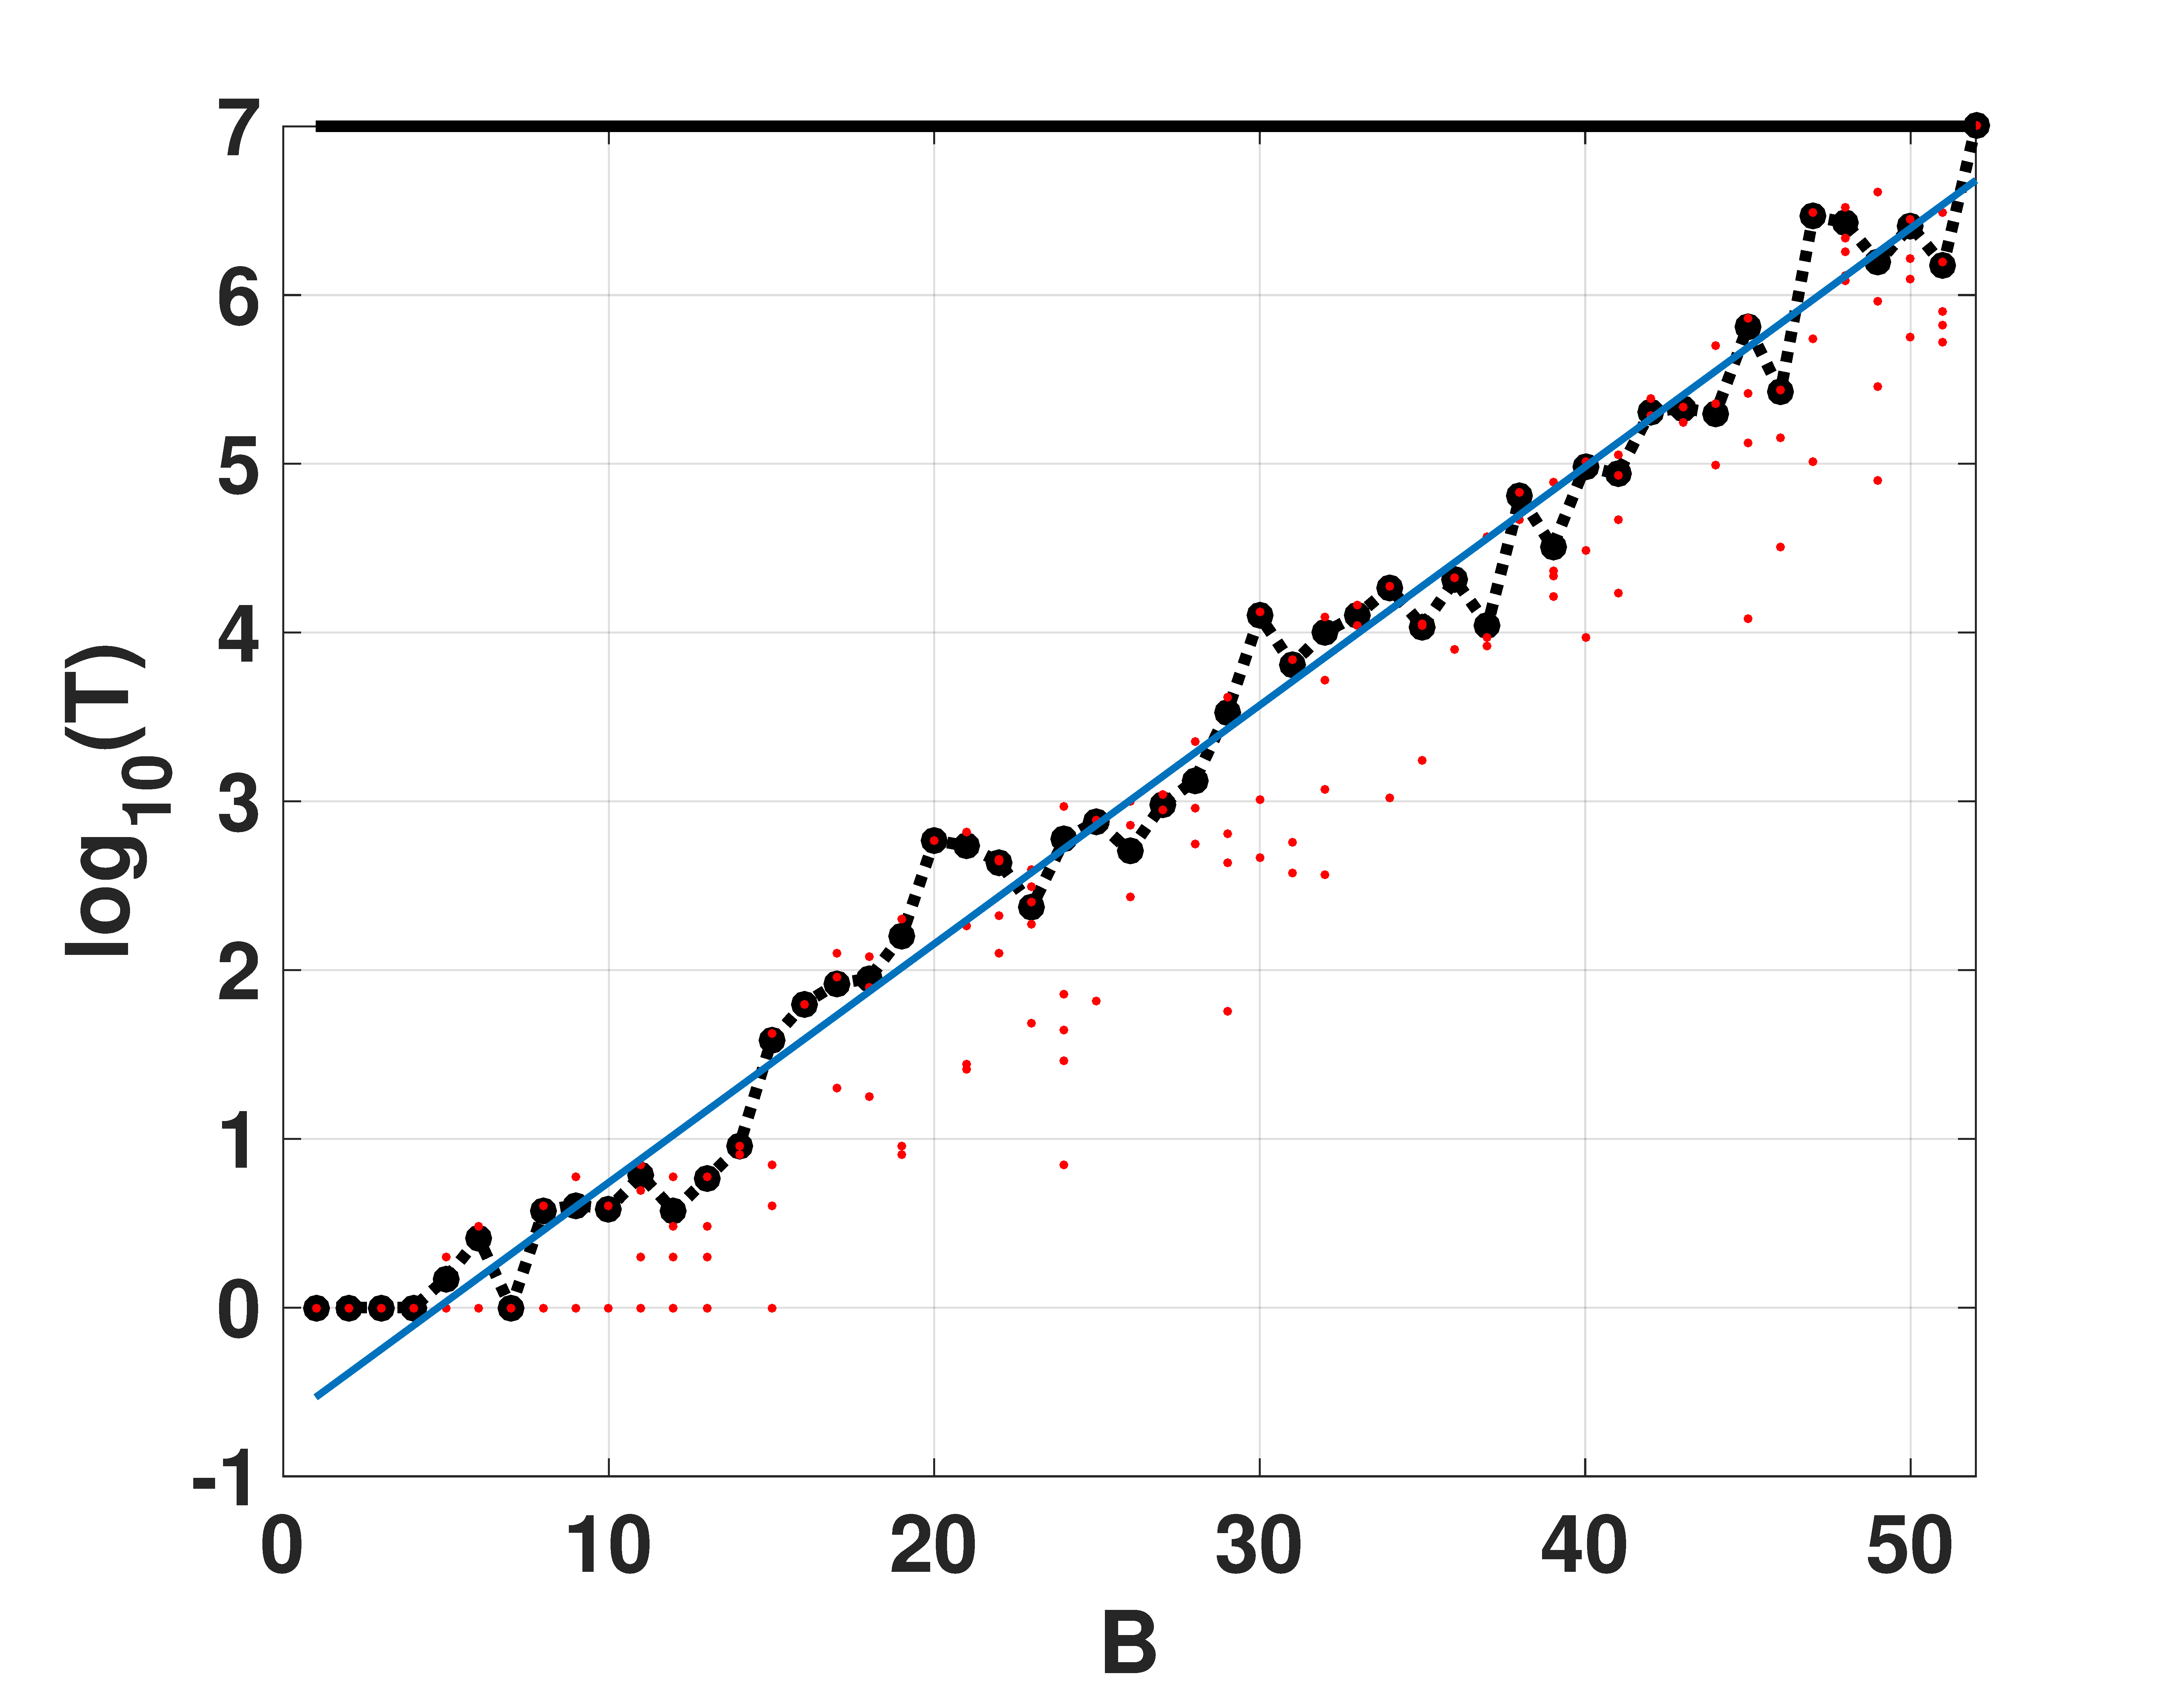
\includegraphics[width=.49\textwidth]{Period_Log}
	\caption{Período $T$ en función de la preceisión $B$ en números binarios para el mapa LOG.} \label{fig:period}
\end{figure}
%
\begin{table}[htpb]
\centering	
	\caption{Período $T$ en función de la preceisión $B$ para todos los mapas considerados}
	\vspace{1em}
	\begin{tabular}{lll}
		\hline\noalign{\smallskip}
		mapa & m & b  \\
		\noalign{\smallskip}\hline\noalign{\smallskip}
		TENT&0 & 0 \\
		LOG &0.139 & -0.6188 \\
		SWITCH &0.1462 & -0.5115 \\
		EVEN &0.1447 & -0.7783 \\
		ODD &0.1444 & -0.7683 \\
		\noalign{\smallskip}\hline
	\end{tabular}
	\label{tabla:periodos}	
\end{table}

Los resultados son compatibles con los obtenidos en \cite{Nagaraj2008}.
La conmutación entre mapas aumenta el período $T$ pero el procedimiento de skipping lo disminuye casi a la mitad.